\documentclass[border=5pt]{standalone}
\usepackage{pgfplots}
\pgfplotsset{compat=1.18}

\begin{document}
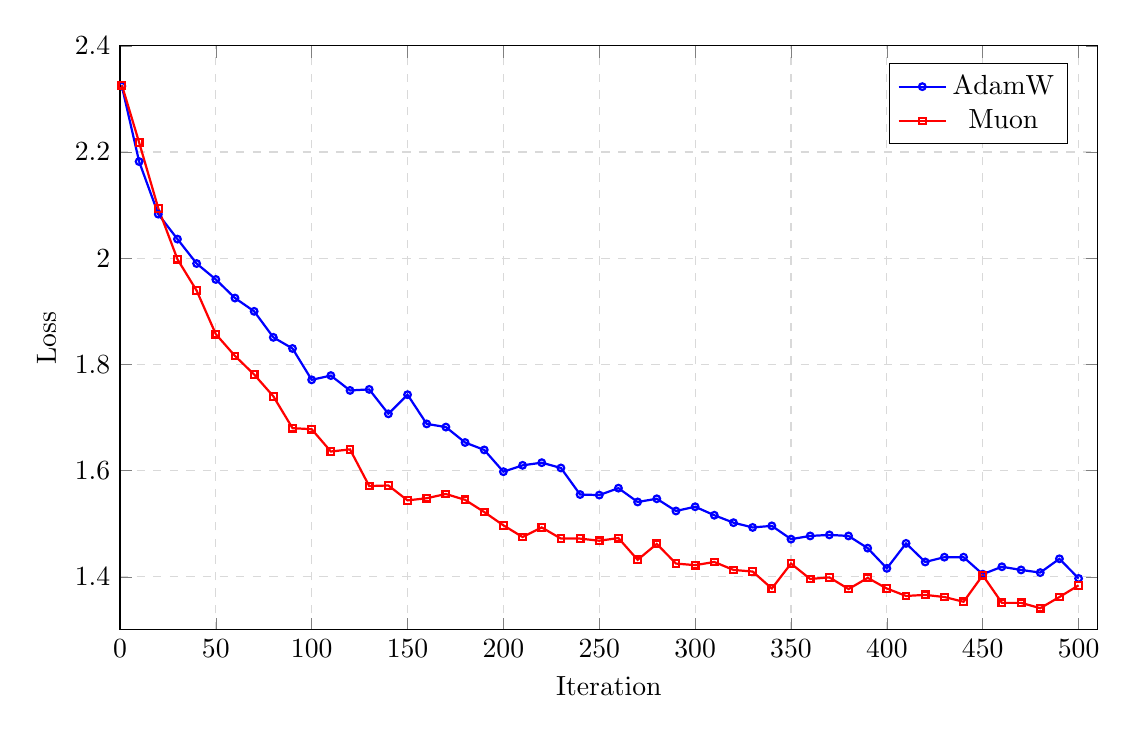
\begin{tikzpicture}
\begin{axis}[
    width=14cm,
    height=9cm,
    xlabel={Iteration},
    ylabel={Loss},
    legend pos=north east,
    grid=major,
    grid style={dashed,gray!30},
    xmin=0, xmax=510,
    ymin=1.3, ymax=2.4,
]

\addplot[blue, thick, mark=o, mark size=1.2pt] coordinates {
    (1,2.324) (10,2.182) (20,2.083) (30,2.036) (40,1.990) (50,1.960) (60,1.925) (70,1.900) (80,1.851) (90,1.830) (100,1.771) (110,1.779) (120,1.751) (130,1.753) (140,1.707) (150,1.743) (160,1.688) (170,1.682) (180,1.653) (190,1.639) (200,1.598) (210,1.610) (220,1.615) (230,1.605) (240,1.555) (250,1.554) (260,1.567) (270,1.541) (280,1.547) (290,1.524) (300,1.532) (310,1.516) (320,1.502) (330,1.493) (340,1.496) (350,1.471) (360,1.477) (370,1.479) (380,1.477) (390,1.454) (400,1.416) (410,1.463) (420,1.428) (430,1.437) (440,1.437) (450,1.405) (460,1.419) (470,1.413) (480,1.408) (490,1.434) (500,1.397)
};
\addlegendentry{AdamW}

\addplot[red, thick, mark=square, mark size=1.2pt] coordinates {
    (1,2.326) (10,2.218) (20,2.094) (30,1.998) (40,1.939) (50,1.857) (60,1.816) (70,1.781) (80,1.740) (90,1.680) (100,1.678) (110,1.636) (120,1.640) (130,1.571) (140,1.572) (150,1.544) (160,1.548) (170,1.556) (180,1.545) (190,1.522) (200,1.497) (210,1.475) (220,1.493) (230,1.472) (240,1.472) (250,1.468) (260,1.473) (270,1.432) (280,1.462) (290,1.425) (300,1.422) (310,1.428) (320,1.413) (330,1.410) (340,1.378) (350,1.425) (360,1.396) (370,1.399) (380,1.377) (390,1.398) (400,1.378) (410,1.364) (420,1.366) (430,1.362) (440,1.353) (450,1.403) (460,1.351) (470,1.351) (480,1.341) (490,1.362) (500,1.384)
};
\addlegendentry{Muon}

\end{axis}
\end{tikzpicture}
\end{document}
